
\section{Gaussian Process Regression}
\label{sec:intro}

We will consider mainly a regression task.
Let $f(\mathbf{x})$ be some unknown smooth function.
Suppose that we are given a data set
$\mathcal{D} = \{(\mathbf{x}_i, y_i), \mathbf{x}_i \in \mathbb{R}^d, y_i \in
\mathbb{R}\}_{i = 1}^N$
of $N$ pairs of inputs $\mathbf{x}_i$ and outputs $y_i$.
This set we will also call {\em training set}.
We would like to construct an approximation $\hat{f}(\mathbf{x})$
of the function $f(\mathbf{x})$
where outputs $y_i$ are assumed to be noisy with additive i.i.d. Gaussian noise:
\begin{equation}
    \label{eq:model}
      y_i = f(\mathbf{x}_i) + \varepsilon_i, \quad \varepsilon_i \sim \mathcal{N}(0, \sigma_{noise}^2).
\end{equation}
The noise level is usually not known.


GP regression is a Bayesian approach where a prior distribution over continuous functions
is assumed to be a Gaussian Process.
This means that any set of function values $f(\mathbf{x}_1), \ldots, f(\mathbf{x}_N)$
have a joint Gaussian distribution \citep{rasmussen2006gaussian}
\begin{equation}
  \label{eq:regression_problem}
  \mathbf{f} \, | \, \mathbf{X} \sim \mathcal{N}(\boldsymbol{\mu}, \, \mathbf{K}_f),
\end{equation}
where $\mathbf{f} = \begin{pmatrix}f(\mathbf{x}_1) & \ldots & f(\mathbf{x}_N\end{pmatrix}^\top$
is a vector of function values,
$\mathbf{X} = \begin{pmatrix}\mathbf{x}_1 & \ldots & \mathbf{x}_N\end{pmatrix}^\top$ is a matrix of inputs,
$\boldsymbol{\mu} =
\begin{pmatrix}\mu(\mathbf{x}_1) & \ldots & \mu(\mathbf{x}_N)\end{pmatrix}^\top$
is a mean vector for some function $\mu(\mathbf{x})$,
$\mathbf{K}_f = \{ k(\mathbf{x}_i, \mathbf{x}_j) \}_{i, j = 1}^N$ is a covariance matrix.
The value of the function $k(\mathbf{x, x}') = \mathbb{E}\left [
  (f(\mathbf{x}) - {\bm \mu}(\mathbf{x}))(f(\mathbf{x}') - {\bm \mu}(\mathbf{x})')
\right ]$ is the covariance between $f(\mathbf{x})$
and $f(\mathbf{x}')$ and is called the {\em covariance function} or the {\em kernel function}.
We will also write Gaussian process as
\[
  f(\mathbf{x}) \sim \mathcal{GP}({\bm \mu}(\mathbf{x}), k(\mathbf{x, x}')).
\]

In GP regression we assume that $f(\mathbf{x})$ from \eqref{eq:regression_problem}
is a Gaussian Process.
Following a Bayesian approach, we would like to derive the posterior distribution
of a value $y^*$ at some arbitrary point $\mathbf{x}^*$ given the observed data
$(\mathbf{X, y})$.
As the joint distribution of $(y^*, \mathbf{y})$ is Gaussian, the posterior
distribution being conditional is also Gaussian
\begin{equation}
\label{eq:gp_posterior}
    \begin{aligned}
        y^* | \mathbf{X}, \mathbf{y}, \mathbf{x}^* &\sim
        \mathcal{N}(\hat{\mu}(\mathbf{x}^*), \hat{\sigma}^2(\mathbf{x}^*)), \\
        \hat{\mu}(\mathbf{x}^*) &=
        \mu(\mathbf{x}^*) + \mathbf{k}(\mathbf{x}^*)^\top \mathbf{K}_y^{-1}
        (\mathbf{y} - \bm{\mu}), \\
        \hat{\sigma}^2(\mathbf{x}^*) &=
        k(\mathbf{x}^*, \mathbf{x}^*) -
        \mathbf{k}(\mathbf{x}^*)^\top \mathbf{K}_y^{-1} \mathbf{k}(\mathbf{x}^*),
    \end{aligned}
\end{equation}
where $\mathbf{k}(\mathbf{x}^*) = \begin{pmatrix}
k(\mathbf{x}^*, \mathbf{x}_1) & \ldots k(\mathbf{x}^*, \mathbf{x}_N)
\end{pmatrix}^\top$
and
$\mathbf{K}_y = \mathbf{K}_f + \sigma_{noise}^2 \mathbf{I}$.
The posterior mean we use as a prediction and the posterior variance
can be used as an uncertainty estimate of the prediction.
It is common practice to use zero-mean function as it can
be accounted in the kernel function.
\begin{figure}[h]
  \centering
  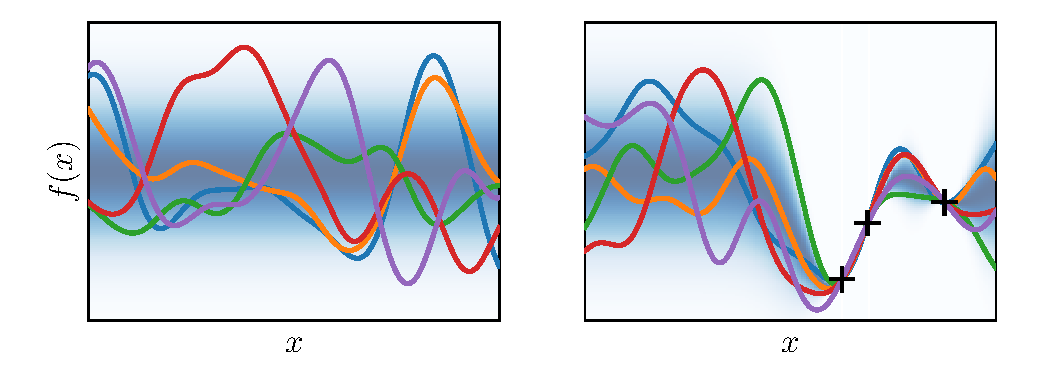
\includegraphics[width=\textwidth]{figures/intro/gp_intro.pdf}
  \caption{Illustration of Gaussian Process Regression in a one-dimensional case.
  The shades of blue represent the distribution of function values at each input point $x$.
  Color lines are random functions sampled from the GP.
  {\em Left}: figure depicts prior distribution over functions with several random
  functions drawn from it.
  {\em Right}: posterior distribution conditioned on several data observations.
  Here the noise in observations is very small, therefore, all posterior samples
  pass through the given points.
  }
  \label{fig:gp_intro}
\end{figure}

The kernel function is central and the most crucial part of GP models.
The type of kernel specifies which class of functions can be approximated by GP
and what peculiarities the model will possess.
By specifying a kernel we can end up with models that are equivalent to other
well known models, like linear regression or splines.
However, in practice usually a squared exponential (it is also often called Radial Basis Function (RBF) kernel) covariance function is used
\begin{equation}
  \label{eq:covariance_function}
  k(\mathbf{x}_p, \mathbf{x}_q) = \sigma_f^2 \exp \left ( -\sum_{i = 1}^d \theta_i^2 (\mathbf{x}_p^{(i)} - \mathbf{x}_q^{(i)})^2 \right ).
\end{equation}
This kernel is infinitely smooth and is shift-invariant,
i.e. $k(\mathbf{x, y}) = k(\mathbf{x - y})$ which has its own advantages and disadvantages.
Nevertheless, this kernel is highly popular and is a universal choice
that works quite well in many applications.


\subsection{Hyperparameters tuning}
One of the appealing property of GP models is that they allow to
carefully tune their hyper-parameters without over-fitting to the observed data.

Let us denote hyper-parameters of the kernel function and noise variance by $\bm{\theta}$.
To choose good $\bm{\theta}$ we consider the log likelihood
\begin{equation}
  \label{eq:loglikelihood}
    \log p(\mathbf{y} \, | \, \mathbf{X}, \boldsymbol{\theta}, \sigma_f, \sigma_{noise}) =
    -\underbrace{\frac12 \mathbf{y}^T \mathbf{K}_y^{-1}\mathbf{y}}_{\text{data fit term}}
    - \underbrace{\frac12 \log |\mathbf{K}_y|}_{\text{complexity term}}
    - \frac{N}{2} \log 2 \pi
\end{equation}
and maximize it over the hyper-parameters \citep{rasmussen2006gaussian}.
The objective is also called {\em marginal log-likelihood} as it implicitly
marginalizes out all function values at other input locations that are not present
in the training set.
There are essentially two terms in the objective function.
One term encourages the data fit and the other one controls the model's complexity.
It allows comparing different models and balance between data interpolation and
the model's capacity.

\section{Features of Gaussian Processes}
GP models have some peculiarities, some of them makes it more attractive, some --- limit their applicability.
\begin{enumerate}
    \item \textbf{Analytical solution}.
      The predictive posterior distribution is given by a simple analytical expression.
      This simplifies analysis of the model and can make it easier to build on top of
      GP model.
      And it is always nice to have a closed-form solution.

    \item \textbf{Marginalization}.
      Marginalization over all function values at locations that are not in the training
      set is actually averaging over a wide range of functions, which
      is actually a strong regularization that makes over-fitting less possible.

    \item \textbf{Flexibility}.
      Different peculiarities of the data set and underlying unknown function
      can be taken into account by considering specific kernel functions.

    \item \textbf{Uncertainty estimation}.
      Predictive distribution allows us to estimate the uncertainty of the prediction.
      It can be required by the application itself as well as used to solve other
      problems, e.g., adaptive Design of Experiments, Bayesian Optimization and others.

    \item \textbf{Well developed theory}.
      GP models have a simple structure and, therefore, have already been
      well studied and many properties have been discovered.
      This makes the models attractive because their behavior can be explained
      theoretically.
      It is also easier to analyze the models that were built on top of GP models.
      Theoretical analysis of the models is essential as it helps to understand
      in what cases the model will or will not work, how to pre-process the data
      or modify the overall approach to make it work and so on.

    \item \textbf{Computational complexity}.
      As it can be seen from \eqref{eq:loglikelihood} we need to calculate the determinant
      and the inverse of the kernel matrix of size $N \times N$.
      Therefore, inference requires $\mathcal{O}(N^3)$ operations, which
      makes it prohibitive to use GP models in case of large data sets.
      Test time evaluation complexity is $\mathcal{O}(N)$ and in some applications it can also
      be too high.
      In Chapter~\ref{chap:gp_on_grids} we show a way to reduce the computational complexity drastically
       for structured data sets,
      and in Chapter~\ref{chap:unstructured_datasets} we consider general unstructured
      data sets and develop an efficient approximation to the kernel function.

    \item \textbf{Kernel choice}. Kernel is the most important part of the GP model.
    It specifies the behavior of the model and a class of functions that can be
    well approximated.
    However, in most cases, we do not know in advance what type of kernel
    best suits the data set at hand and either stick to some universal kernel (like RBF)
    or construct an appropriate kernel manually.
    Nevertheless, there are some works that tries to select the best kernel automatically, for example, \citep{duvenaud2014automatic, abdessalem2017automatic, teng2020scalable}.
    There are works that bypass the kernel design by building Deep Gaussian Processes \citep{damianou2013deep} or
    combine deep networks with Gaussian Processes \citep{wilson2016stochastic}.

    \item \textbf{Gaussian distribution}.
    In GP the distribution of output values (i.e., likelihood) is Gaussian.
    Sometimes the actual likelihood is non-Gaussian, for example, when we deal
    with classification tasks.
    In this case we need to use approximate solutions.
    This direction is well developed and there are several frameworks
    that allows us to work with non-Gaussian likelihoods \citep{de2017gpflow,gardner2018gpytorch} easily.

\end{enumerate}

In the thesis we approach the computational complexity issue.
There is considerable amount of work in this direction
(for example, \citep{quinonero2005unifying,rahimi2008random,titsias2009variational,cutajar2017random}).
Nevertheless, we would like to point that
generally exact Gaussian Process models work better than the existing approximations
\citep{cutajar2016preconditioning,wang2019exact}.
Also, typically large-scale approximate methods have hyper-parameter that controls
the accuracy of the approximation (for example, number of inducing points in \citep{quinonero2005unifying,titsias2009variational}
and number of features in \citep{rahimi2008random,felix2016orthogonal} and their follow-ups).
The analysis of such approaches show that optimal learning rates requires this parameter to be at least $\mathcal{O}(\sqrt{N} \log N)$
\citep{aless2016generalization,rudi2017falkon}.
Therefore, the computational complexity becomes $\mathcal{O}(N\sqrt{N})$ in this case.
In the thesis we prefer to do exact inference when it is possible.
In case of large-scale data sets it can be done if there is a way
to exploit the structure of the problem.
Such approach we develop in Chapter \ref{chap:gp_on_grids} for data sets on multi-dimensional grids
and show that its computational complexity is lower than the complexity of the large-scale approximations.


In case of unstructured data sets the way to build large-scale Gaussian Process model
is to do approximations.
Current state-of-the-art scalable approaches show great effectiveness in real-world
problems.
Better performance is usually achieved by {\em data-dependent} approaches, i.e.
the approaches that rely on the given data set.
On the other hand, in some applications {\em data-independent} techniques are more attractive as
they do not require the data set to construct an approximation.
For example, applications where we data changes frequently, so it is more costly
or less accurate to use data-dependent techniques.
Simultaneous localization and mapping is an example of such problems (we consider it Chapter \ref{chap:applications}).
For this reasons in the thesis we focus on data-independent approach.




